\documentclass[11pt, a4paper]{article}

\usepackage[czech]{babel}
% \usepackage[IL2]{fontenc} % pro iso8859-2
\usepackage[utf8]{inputenc}   % pro unicode UTF-8

\newcommand{\Author}{Tomáš Báča}
\newcommand{\Title}{Řídicí deska multikopter}
\newcommand{\Acronym}{Acronym}
\newcommand{\WorkPackage}{WorkPackage}
\newcommand{\DocName}{Technický manuál}
\newcommand{\Subject}{\WorkPackage - \DocName}
\newcommand{\Keywords}{mobile robotics}
\newcommand{\Date}{11/07/2011}
\newcommand{\DOCVersion}{0.1}

\pdfoutput=1
\documentclass[a4paper,12pt,titlepage, twoside]{article}


\usepackage[english]{babel}
\usepackage[utf8]{inputenc}
\usepackage{amssymb,amsmath}
\usepackage{algorithm,algpseudocode}
\usepackage[title,titletoc]{appendix}
\usepackage{latexsym}
\usepackage{a4wide}
\usepackage{color} 
\usepackage{indentfirst}
\usepackage{graphicx}       %%% graphics for dvips
\usepackage{fancyhdr}
\usepackage{longtable}
\usepackage{pifont}
\usepackage{makeidx}
\usepackage{lastpage}
\usepackage{multirow}
\usepackage{dcolumn} 
\usepackage{epstopdf}
\usepackage{url}
\usepackage{listings}
\usepackage{caption}
\usepackage{subcaption}
\usepackage{relsize}
\usepackage{pdfpages}
\usepackage{rotating}
\usepackage{natbib}
\usepackage{cite}
\usepackage{booktabs}
\usepackage[table,xcdraw]{xcolor}

\newcommand{\Author}{Jiří Fiedler}
\newcommand{\Title}{MAV communication protocol}
\newcommand{\Acronym}{Acronym}
\newcommand{\WorkPackage}{WorkPackage}
\newcommand{\DocName}{MAV communication protocol}
\newcommand{\Subject}{\WorkPackage - \DocName}
\newcommand{\Keywords}{mobile robotics}
\newcommand{\Date}{11/05/2015}
\newcommand{\DOCVersion}{1.0}

% European layout (no extra space after `.')
\frenchspacing

% nastavení výstupu
\def\nothtml{}  					%%% \nothtml is defined if not processed with latex2html
\usepackage[                		%%% hyper-references for ps2pdf
bookmarks=true,%                   	%%% generate bookmarks ...
breaklinks=true,%                  	%%% breaks lines, but links are very small
hypertexnames=false,%              	%%% needed for correct links to figures
colorlinks=false,%
urlcolor=blue
]{hyperref}           				%%% blue instead of cyan URLS
\hypersetup{
pdfcreator  = {LaTeX with hyperref package},
pdfproducer = {dvips + ps2pdf},
colorlinks=false,
pdfborder={0 0 0},
}

\hypersetup{  
pdfauthor={\Author},
pdftitle={\Title - \Acronym},
pdfsubject={\Subject},
pdfkeywords={\Keywords}}

% úpravy vzhledu stránek
\setlength{\headheight}{18pt}			%%% drobně odsadí hlavičku
\renewcommand{\footrulewidth}{0.4pt}  	%%% horizontal line in footer
\fancyhead[R]{} 						%%% umaže pravou stranu hlavičky

\newcommand{\jed}[1]{\ensuremath{~\mathrm{#1}}} %příkaz pro sazbu fyzikálních jednotek
\newcommand{\dd}[1]{\ensuremath{\mathrm{d}#1}} %příkaz pro sazbu diferenciálu
\newcommand{\EE}[1]{\ensuremath{ \cdot 10^{#1}}} %příkaz pro sazbu *10^x

\newcommand{\pd}[2]{\ensuremath{\frac{\partial #1}{\partial #2}}} %parc. derivačka

\begin{document}

\begin{titlepage}

\begin{center}

\textsc{\LARGE České vysoké učení technické v Praze }\\[1.0cm]
\textsc{\LARGE Fakulta elektrotechnická }\\[1.0cm]
\textsc{\large Skupina inteligentní a mobilní robotiky }\\[0.5cm]

% Title
%\HRule \\[5.0cm]
{ \huge \bfseries Simulátor letounů\\[0.5cm] návod v.1 }\\[1.0cm]
%\HRule \\[1.5cm]

% Author and supervisor
\large
\textsc{\Author}

\vfill

\end{center}

\end{titlepage}

\newpage

\tableofcontents

\newpage

\setlength{\parskip}{0.35cm}
\pagenumbering{arabic}
\lhead{\emph{\leftmark}}
\rhead{}
\cfoot{}
\rfoot{\thepage$/$\pageref{LastPage}}

\section{Instalace simulátoru}

Instalace nevyžaduje zvláštní instrukce. Po instalaci spusťte simulátor a proklikejte se úvodními informacemi, než se zobrazí obrazovka s žádostí o připojení USB adapteru (Obrázek~\ref{fig:obr1}).

\section{Připojení RC vysílače}

\begin{figure}[h]
\begin{center}
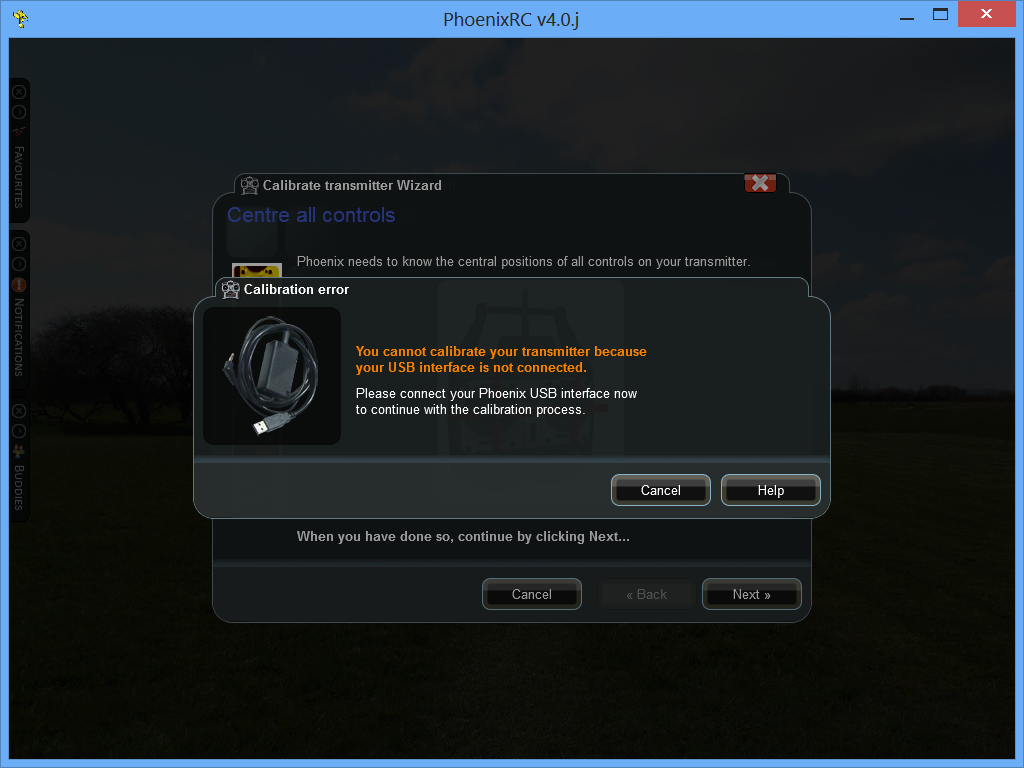
\includegraphics[width=0.8\textwidth]{fig/1.PNG}
\caption{Není připojen USB adapter}
\label{fig:obr1}
\end{center}
\end{figure}

Po připojení USB adapteru si simulátor začne zjišťovat přítomnost RC vysílačky připojené do adapteru. Pokud nebude připojená, nebo nebude aktivovaná funkce pro komunikace po kabelu, zobrazí se obrazovka s příslušnou informací (Obrázek~\ref{fig:obr2}).

\begin{figure}[h]
\begin{center}
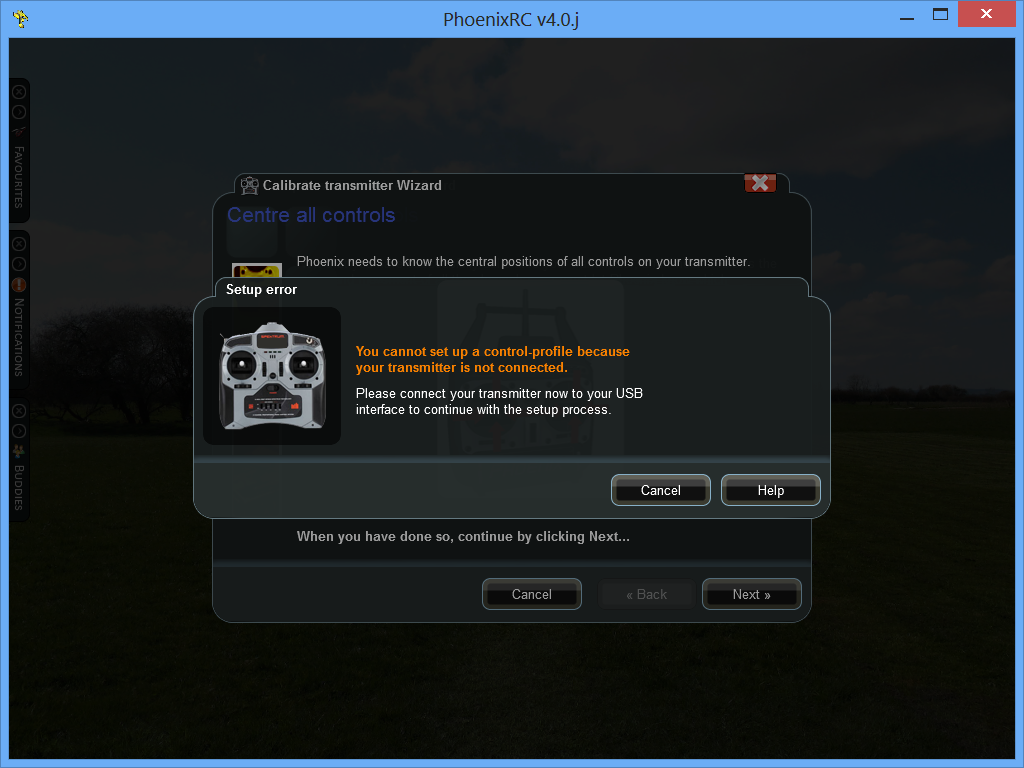
\includegraphics[width=0.8\textwidth]{fig/2.PNG}
\caption{Není připojena RC vysílačka}
\label{fig:obr2}
\end{center}
\end{figure}

Po připojení konektoru z USB adapteru do RC vysílačky ji zapněte. Vyčkejte na zobrazení úvodní obrazovky. Pokud je USB adapter zapojen do PC, v pravém dolním rohu displeje RC vysílače se objeví tlačítko s nápisem \textbf{Multi-I/O} (Obrázek~\ref{fig:obr3}).

\begin{figure}[h]
\begin{center}
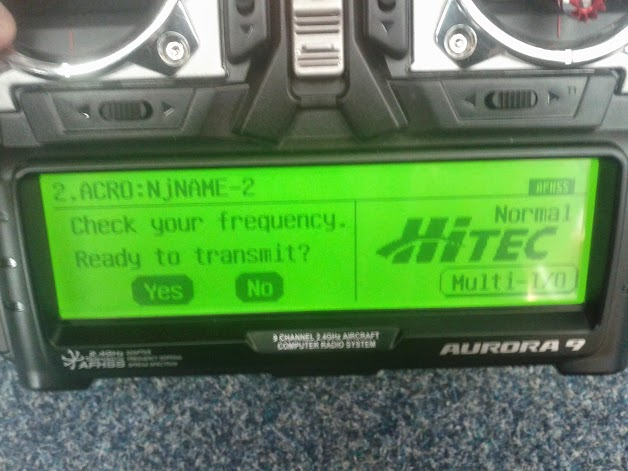
\includegraphics[width=0.8\textwidth]{fig/rc1.jpg}
\caption{Úvodní obrazovka RC vysílače}
\label{fig:obr3}
\end{center}
\end{figure}

Po stisknutí tlačítka \textbf{Multi-I/O} se objeví obrazovka se dvěma dalšími tlačítky (Obrázek~\ref{fig:obr4}). Zde stiskněte tlačítko \textbf{T.Pupil}. Tím přepnete vysílačku do režimu, kdy posílá data po kabelu do PC.

\begin{figure}[h]
\begin{center}
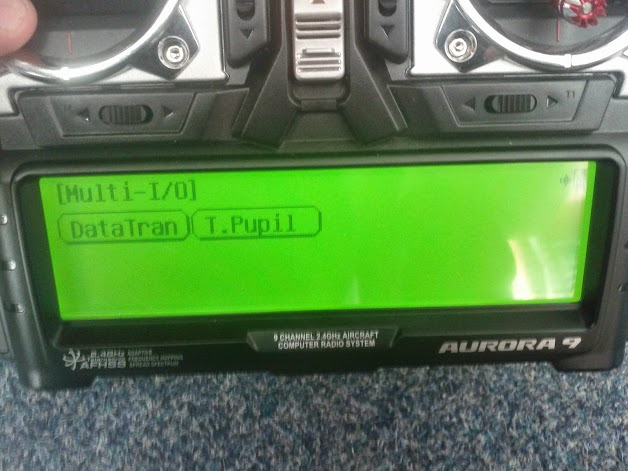
\includegraphics[width=0.8\textwidth]{fig/rc2.jpg}
\caption{Druhá obrazovka RC vysílače}
\label{fig:obr4}
\end{center}
\end{figure}

\section{Kalibrace vysílače}

Při první připojení vysílače k simulátoru je potřeba nakalibrovat páky. Simulátor Vás na tuto skutečnost upozorní příslušnou obrazovkou (Obrázek~\ref{fig:obr5}).

\begin{figure}[h]
\begin{center}
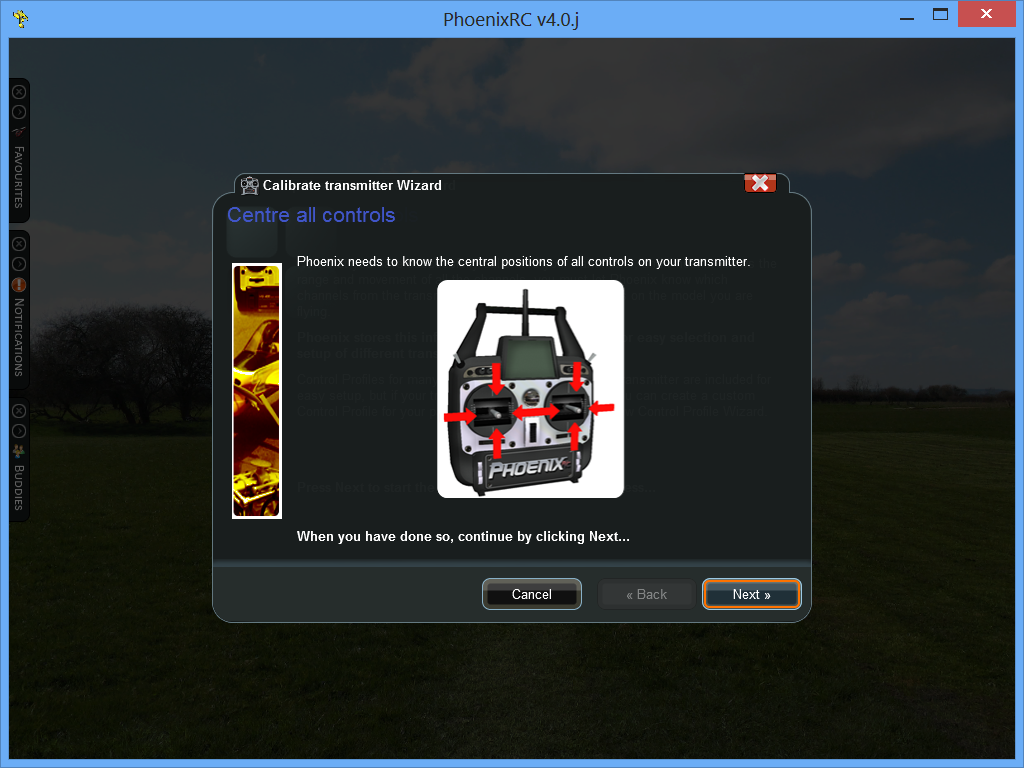
\includegraphics[width=0.8\textwidth]{fig/3.PNG}
\caption{Kalibrace vysílače, umístěte hlavní páky do středových poloh}
\label{fig:obr5}
\end{center}
\end{figure}

Dále po vás bude vyžadovat pohnutím obou hlavních pák do všech krajních poloh (Obrázek~\ref{fig:obr6}). Tímto si simulátor zjistí skutečné minimální a maximální hodnoty pák. Až se budou sloupce plynule měnit z min do max, přejděte na další obrazovku.

\begin{figure}[h]
\begin{center}
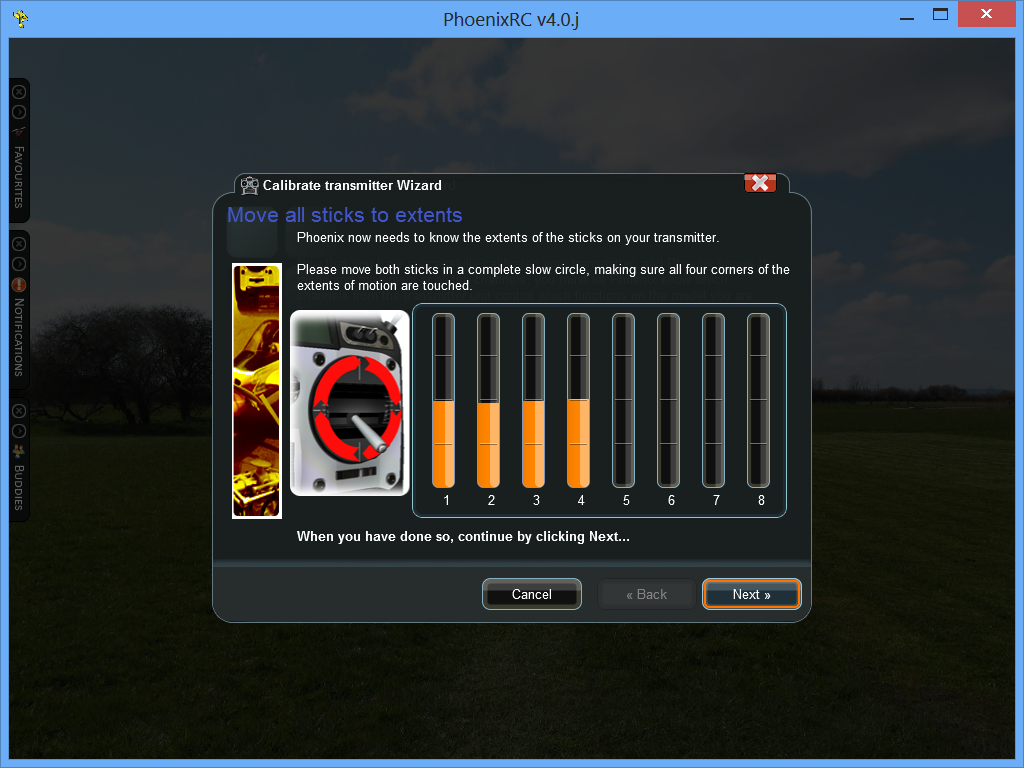
\includegraphics[width=0.8\textwidth]{fig/4.PNG}
\caption{Hýbejte hlavními pákami do všech krajních hodnot}
\label{fig:obr6}
\end{center}
\end{figure}

Následující obrazovka po Vás chce projít ostatní páky a přepínače do krajních poloh, toto \textbf{není} třeba dělat.

Další obrazovka Vám nabídne možnost zkontrolovat předchozí nastavení. Zkontrolujte, že krajní hodnoty obou hlavní pák se shodují s krajními hodnotami příslušných 4 sloupců.

\section{Nastavení ovládání (interpretace signálů z vysílače)}

Na následující obrazovce (Obrázek~\ref{fig:obr7}) je třeba vybrat správný typ vysílače, kterým je Hitec Aurora 9. Poté, co se přesunete do hlavního prostředí simulátoru je potřeba ještě přiřadit signálům z vysílače správné ovládací prvky simulovaného letounu. To se provede v menu \textbf{System~-~Your controls} (Obrázek~\ref{fig:obr8}).

\begin{figure}[h]
\begin{center}
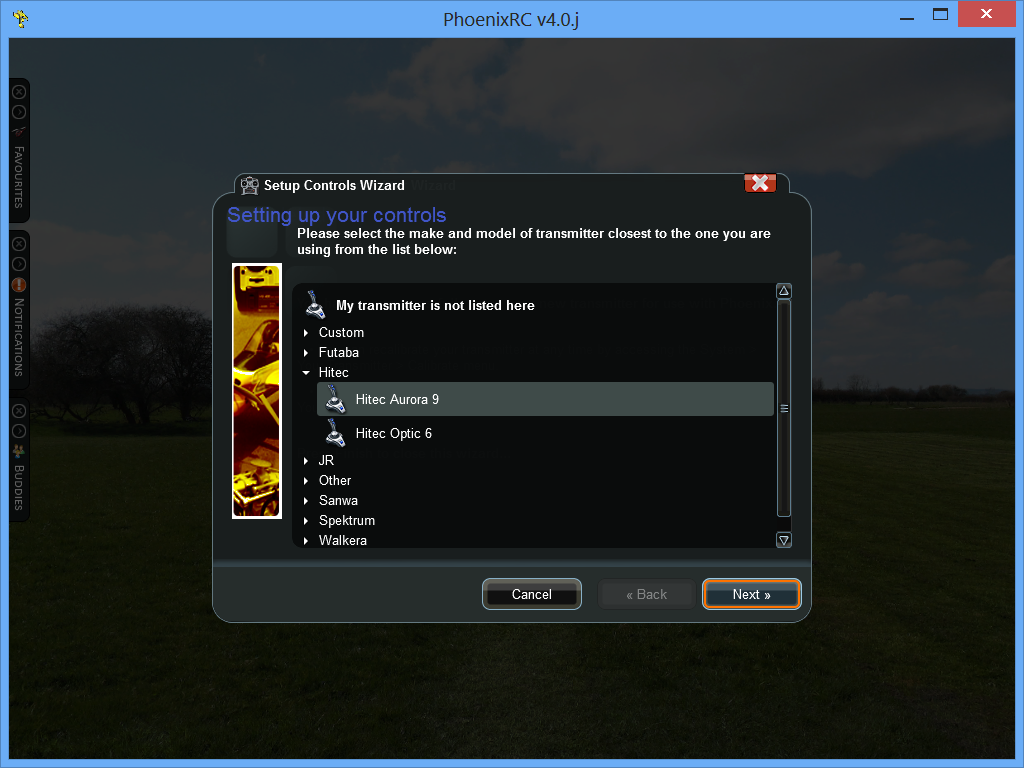
\includegraphics[width=0.8\textwidth]{fig/7.PNG}
\caption{Výběr vysílače Aurora 9}
\label{fig:obr7}
\end{center}
\end{figure}

\begin{figure}[h]
\begin{center}
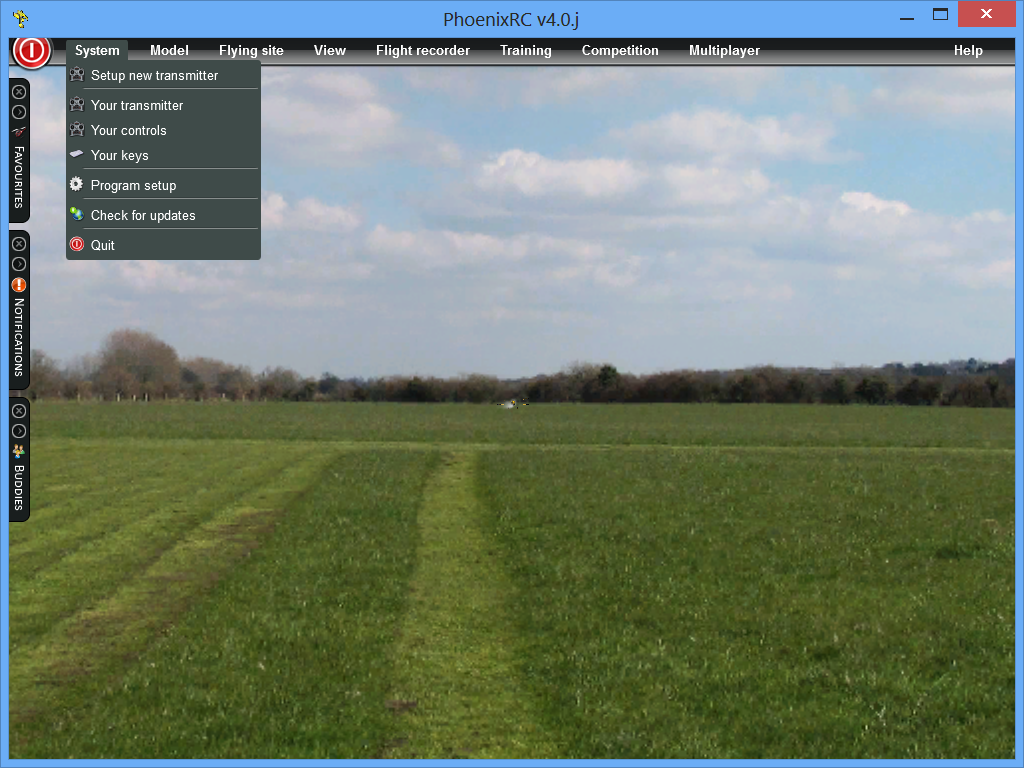
\includegraphics[width=0.8\textwidth]{fig/8.PNG}
\caption{Menu programu}
\label{fig:obr8}
\end{center}
\end{figure}

Následně upravte nastavení vysílače \textbf{Hitec Aurora 9} (Obrázek~\ref{fig:obr9}).

\begin{figure}[h]
\begin{center}
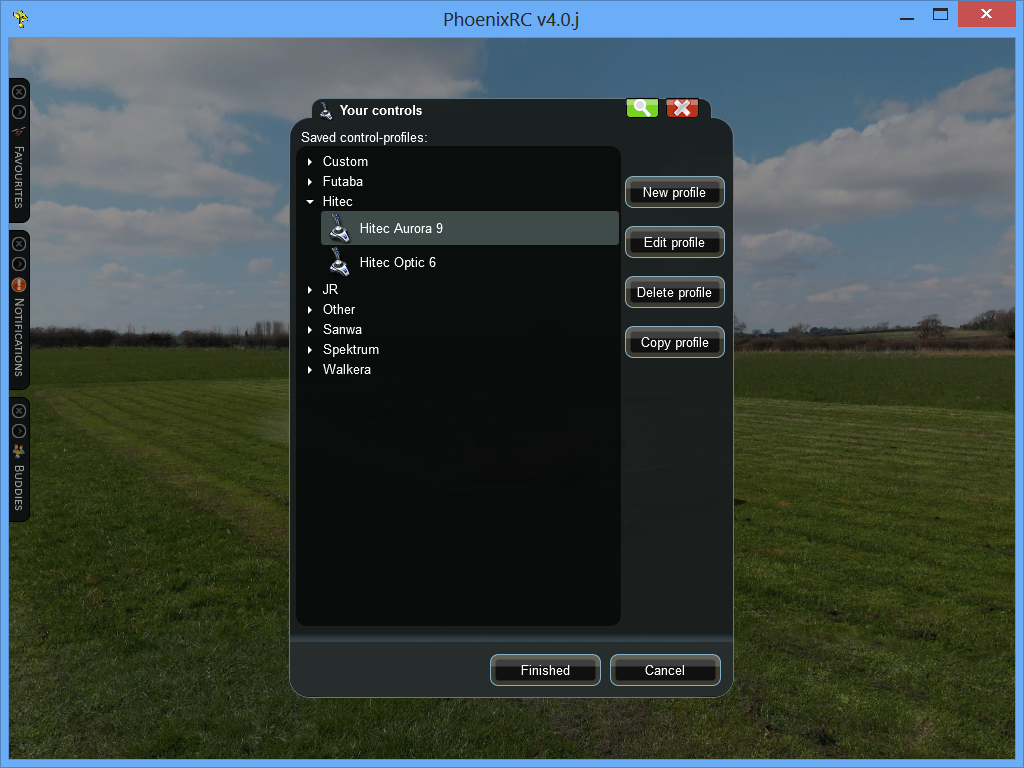
\includegraphics[width=0.8\textwidth]{fig/9.PNG}
\caption{Úprava nastavení Hitec Aurora 9}
\label{fig:obr9}
\end{center}
\end{figure}

Poté je potřeba ke každému ze čtyř řídicích signálů (Enegine, Elevator, Aileron, Rudder) přiřadit správný kanál z RC vysílače. Hodnota sloupce \textbf{Invert} bude zaškrtnutá pouze u signálu Elevator. Nastavení by mělo vypadat stejně, jako na Obrázku~\ref{fig:obr10}. Ve stejném menu doporučuji nastavit nelineární křivky přenosu z vysílače na řídicí signály. To se provede tlačítkem ve sloupci \textbf{Curve} u příslušného signálu (Elevator a Aileron). Pro začátečníky doporučuji 50\% exponencielní křivku, která udělá stroj citlivější u středových pozic pák (Obrázek~\ref{fig:obr11}).

\textbf{Pozor!} Může se stát, že simulátor nebude chtít nastavení profilu vysílače uložit, namísto toho udělá kopii profilu. V takovém případě poté vždy upravujte příslušnou kopii. 

\begin{figure}[h]
\begin{center}
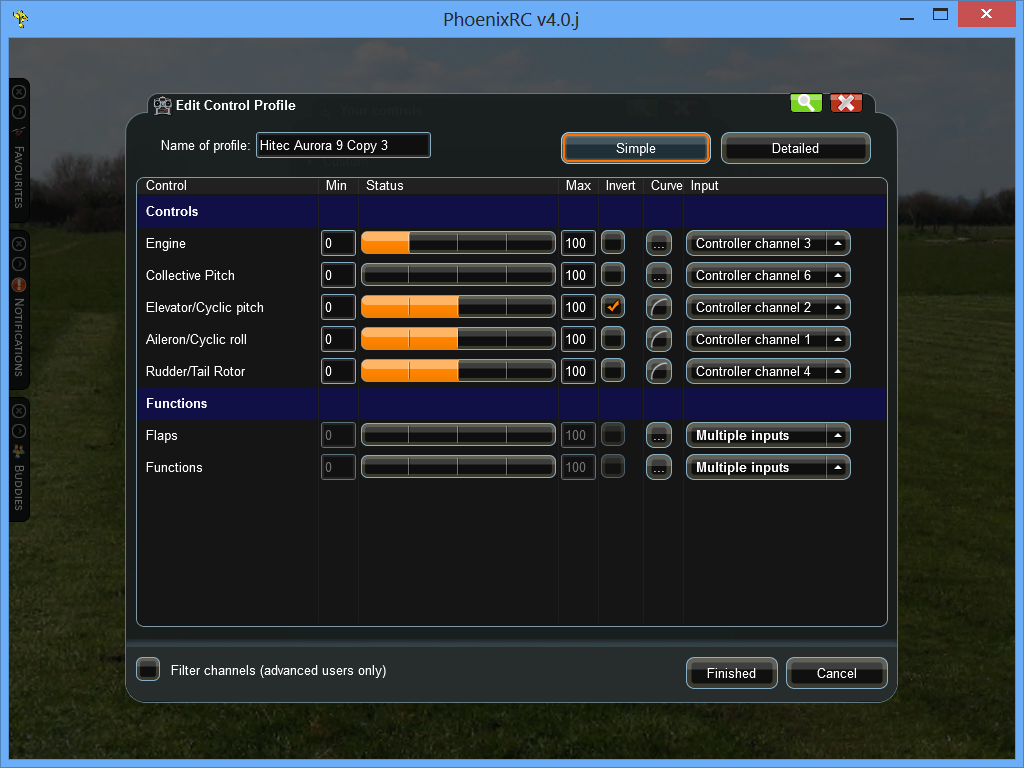
\includegraphics[width=0.8\textwidth]{fig/10.PNG}
\caption{Přiřazení kanálů z vysílače k řídicím signálům simulátoru}
\label{fig:obr10}
\end{center}
\end{figure}

\begin{figure}[h]
\begin{center}
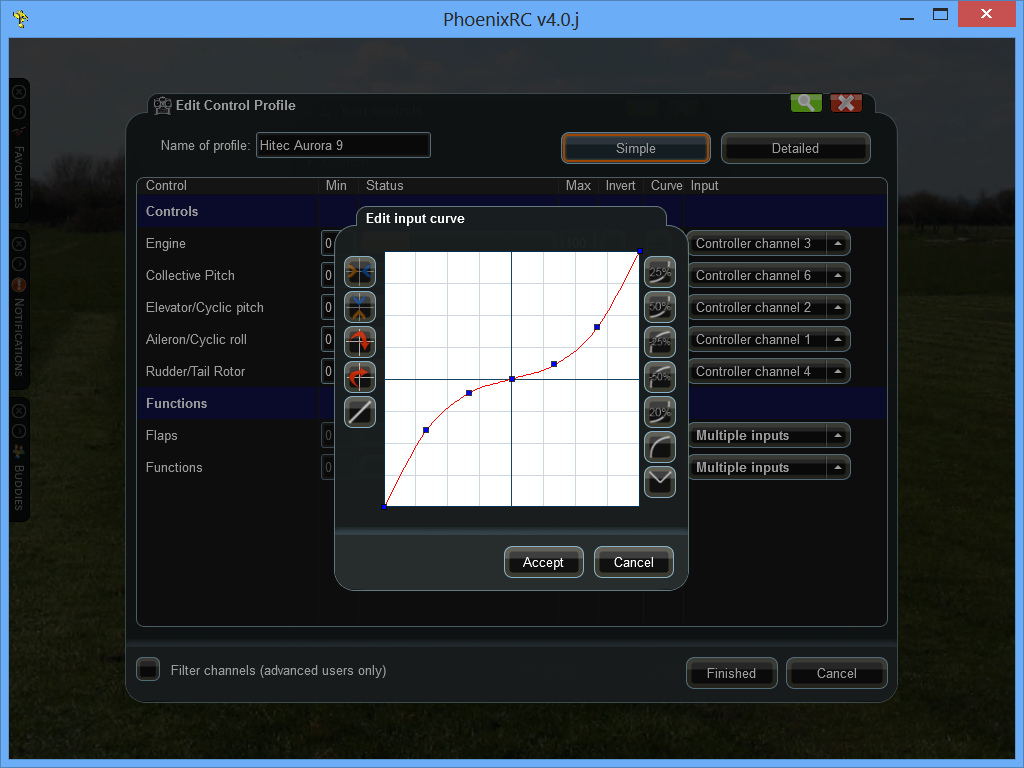
\includegraphics[width=0.8\textwidth]{fig/11.PNG}
\caption{Nastavení křivky přenosu z páky na signál}
\label{fig:obr11}
\end{center}
\end{figure}

Dále v menu \textbf{Model - Change} vyberte model kvadrukoptery (Obrázek~\ref{fig:obr12}). Žlutá kulička u modelu značí předek letounu. Pro naprosté začátečníky doporučuji začít s tréninkem za pomocí módu v menu \textbf{Training - Hover Training}, kdy Vám simulátor zafixuje výšku a některé další osy.

\begin{figure}[h]
\begin{center}
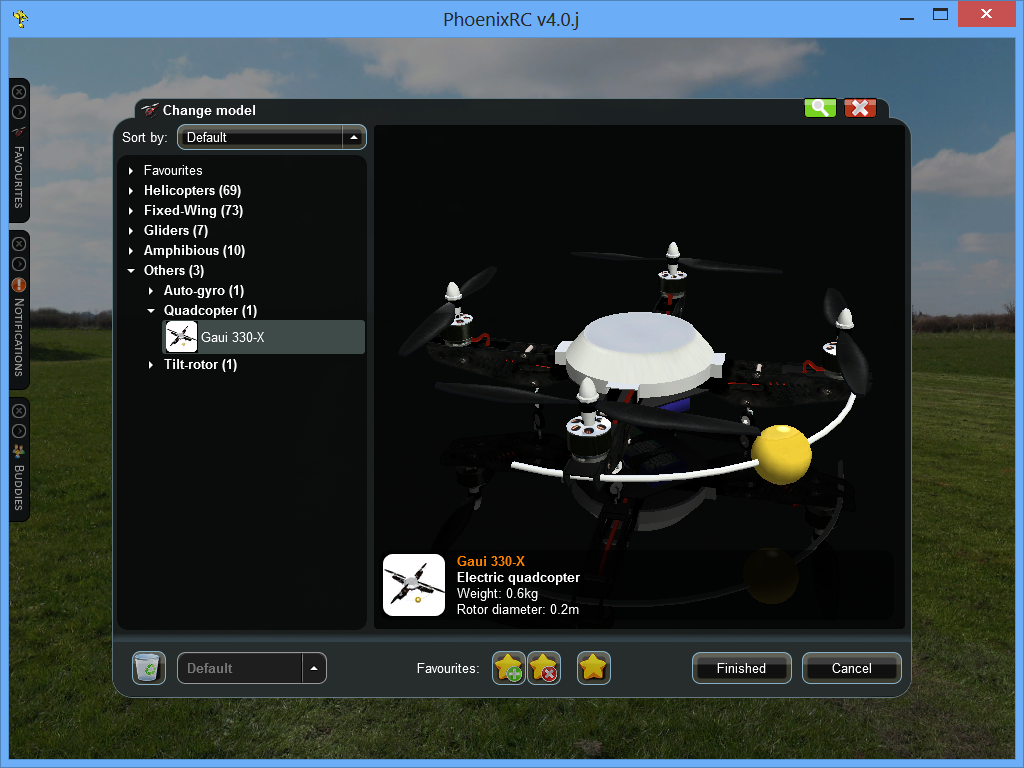
\includegraphics[width=0.8\textwidth]{fig/13.PNG}
\caption{Model kvadrukoptery}
\label{fig:obr12}
\end{center}
\end{figure}

\end{document}